\documentclass[letterpaper,twocolumn]{article}

\usepackage[top=1in,bottom=1in,left=0.75in,right=0.75in]{geometry}
\usepackage{graphicx}
\usepackage{newtxtext}
\usepackage{newtxmath}
\usepackage[hyphens]{url}

% Better look for citations that include a section reference like \cite[\S 3]{foobar}.
\usepackage{cite}
\renewcommand{\citemid}{~}

% Load hyperref after other packages.
\usepackage[pdfa,hidelinks,pdfcreator={},pdfproducer={}]{hyperref}
\urlstyle{same}
\def\sectionautorefname{Section}
\def\subsectionautorefname{Section}

% Disable metadata for reproducible PDF.
% https://tex.stackexchange.com/a/313605
\usepackage{ifpdf}
\ifpdf
\pdfinfoomitdate=1
\pdftrailerid{}
\pdfsuppressptexinfo=-1
\fi

\hyphenation{Web-RTC}
\hyphenation{Java-Script}

\begin{document}

\date{}

\title{Snowflake, a peer-to-peer censorship circumvention system}

% ANON
\author{}

\maketitle

\begin{abstract}
\begin{itemize}
\item temporary proxies using WebRTC
\item central matching of proxies and clients
\item JavaScript browser add-on, or command-line proxies
\item deployed in Tor Browser
\item history of deployment and blocking attempts
\item observations for circumvention
\end{itemize}
\end{abstract}

% General references:
%   https://gitlab.torproject.org/tpo/anti-censorship/pluggable-transports/snowflake/-/wikis/Technical%20Overview
%   https://www.bamsoftware.com/papers/thesis/#chap:snowflake

\section{Introduction}
\label{sec:intro}

Put Snowflake in context

Spectrum of looks-like-nothing to looks-like-something

Spectrum of few, valuable proxies with careful distribution to
many, cheap proxies with less emphasis on secrecy

\section{Background}
\label{sec:background}

% serene, david

WebRTC

% hooman
- interacting suite of multiple protocols
- example applications
- importantly: built into browsers

flash proxy~\cite{Fifield2012a} (\url{https://bugs.torproject.org/legacy/trac/5578})
% flashproxy.pdf §5.2: "New technologies like WebRTC [24] may fill this need in the future, if they become sufficiently popular that flash proxies' use of them does not stand out as unusual."
uProxy (\url{https://serene.cx/snowflake/})

Comparison with MassBrowser~\cite{Nasr2020a}
% https://github.com/net4people/bbs/issues/32

\section{How it works}

% serene, arlo

\begin{figure*}
\framebox[\textwidth]{\vbox to 2in{\vfil\centering TODO\vfil}}
\caption{
Architecture of Snowflake.
}
\label{fig:architecture}
\end{figure*}

\autoref{fig:architecture}

Centralized broker, manages associations between clients and proxies

% hooman
Centralized bridge
- (notionally centralized, though may be realized as multiple instances for performance reasons, see \autoref{sec:experience})

Decentralized proxies
- Clients do not touch the bridge directly, but only through a proxy
- No risk if the bridge itself is blocked
- Proxies can be blocked---even in the middle of an ongoing connection---and clients can adapt by switching to another proxy
- In practice, realized as browser add-ons or standalone executables

Many moving parts, managing complexity is a consideration

\subsection{Rendezvous}

% serene

Communication with broker has different anti-blocking requirements,
can be slower / more expensive

Contents of rendezvous messages
WebRTC signaling, ICE as part of WebRTC
requires bidirectional

Domain fronting remains an important element of circumvention systems,
though since the reaction by cloud providers
to the attempted blocking of Telegram in Russia in 2018,
% TODO: cite something
% From https://gitlab.torproject.org/tpo/network-health/metrics/timeline:
% |2018-04-13 16:00:00|||snowflake|Snowflake client registrations (based on domain fronting) stop working, because of a Google infrastructure change that stops domain fronting from working. The time of the change is between 2018-04-13 14:00:00 and 2018-04-13 18:00:00, based on when the bandwidth graph of the Snowflake bridge [5481936581E23D2D178105D44DB6915AB06BFB7F](https://metrics.torproject.org/rs.html#details/5481936581E23D2D178105D44DB6915AB06BFB7F) went to zero.|[ticket](https://bugs.torproject.org/tpo/anti-censorship/pluggable-transports/snowflake/25804)||
% |2018-04-16|||snowflake|Moved the Snowflake broker from App Engine to a standalone server.|[comment](https://bugs.torproject.org/tpo/anti-censorship/pluggable-transports/snowflake/22874#note_2591708)||
% |2018-05-09 20:46:16|||snowflake|Release of Tor Browser 8.0a7, which changes the default Snowflake rendezvous to use an Azure domain front, instead of the Google one that had been non-functional since 2018-04-13.|[blog post](https://blog.torproject.org/tor-browser-80a7-released) [ticket](https://bugs.torproject.org/tpo/applications/tor-browser/26010)||
it is recognized that domain fronting should not be relied on exclusively.


domain fronting
AMP cache
others?
- DNS over encryption
- flash proxy could use email

long polling

\subsection{Temporary proxying}
\label{sec:proxying}

% cecylia

Proxies are simple conduits, transferring a reliable stream between endpoints
End-to-end security between client and bridge, proxies untrusted

% david
Turbo Tunnel~\cite{Fifield2020a}
KCP/smux
- session layer independent of the circumvention channel, permits switching proxies on the fly
- the protocol layering generally

Web badge vs. browser add-on vs. standalone daemon
majority browser add-on, more effective at gaining popularity than web badge

% cecylia
NAT type matching (necessity of, and how it works)
probetest

\subsection{Protocol fingerprinting}

% kyle, david

\url{https://gitlab.torproject.org/tpo/anti-censorship/pluggable-transports/snowflake/-/wikis/Fingerprinting}

Fifield and Gil Epner~\cite{arxiv.1605.08805}

MacMillan et~al.~\cite{arxiv.2008.03254}

Snowflake leans heavily into the ``address blocking'' side of blocking
resistance, but the ``content blocking'' part is still important.

Fingerprintable features
- signaling
- STUN (choice of servers and contents of messages)
- DTLS
- WebRTC media channel vs. data channel

Historically overvalued in research (cf. \cite{Tschantz2016a})
Practicality is paramount; censors are hard to predict
But we can anticipate possible reactions

\section{Experience}
\label{sec:experience}

\subsection{Deployment history}

% Excerpts from https://gitlab.torproject.org/tpo/network-health/metrics/timeline:
% |2017-01-24|||snowflake|Tor Browser 7.0a1 released, including Snowflake for GNU/Linux only.|[blog post](https://blog.torproject.org/blog/tor-browser-70a1-released)||
% |2017-08-08|||snowflake|Tor Browser 7.5a4 released, including Snowflake for macOS.|[blog post](https://blog.torproject.org/blog/tor-browser-75a4-released) [issue](https://bugs.torproject.org/tpo/applications/tor-browser/22831)||
% |2018-03-26 20:43:42|||snowflake|Release of Tor Browser 8.0a5. Improves snowflake client performance.|[blog post](https://blog.torproject.org/tor-browser-80a5-released) [ticket](https://bugs.torproject.org/tpo/anti-censorship/pluggable-transports/snowflake/21312)||
% |2019-10-01|||snowflake|Release of Tor Browser 9.0a7, the first release that has Snowflake for Windows.|[blog post](https://blog.torproject.org/new-release-tor-browser-90a7) [ticket](https://bugs.torproject.org/tpo/anti-censorship/pluggable-transports/snowflake/25483)||
% |2020-05-22 19:51:29|||snowflake|Release of Tor Browser 9.5a13, the first release with Turbo Tunnel session persistence features for Snowflake. There is a spike in estimated users on 2020-05-21 and 2020-05-22, which appears to be an artifact.|[blog post](https://blog.torproject.org/new-release-tor-browser-95a13) [ticket](https://bugs.torproject.org/tpo/applications/tor-browser/34043) [users graph](https://metrics.torproject.org/userstats-bridge-transport.html?start=2020-03-01&end=2020-08-01&transport=snowflake)||
% |2020-06-02 18:09:48|||snowflake|Release of Tor Browser 10.0a1, the first release with Snowflake for Android.|[blog post](https://blog.torproject.org/new-release-tor-browser-100a1) [ticket](https://bugs.torproject.org/tpo/applications/tor-browser/30318)||
% |2020-06-25|2020-06-25||snowflake|One- or two-day spike in estimated Snowflake users. It resembles the spike that occurred around the time of the Turbo Tunnel release of Tor Browser 9.5a13 on 2020-05-22.|[users graph](https://metrics.torproject.org/userstats-bridge-transport.html?start=2020-03-01&end=2020-08-01&transport=snowflake)|X|
% |2021-07-06 16:56:37|||snowflake|Release of Tor Browser 10.5, first stable release that includes Snowflake.|[blog post](https://blog.torproject.org/new-release-tor-browser-105)||
% |2021-12-20|||snowflake|Release of Tor Browser 11.0.3, with an altered DTLS fingerprint in Snowflake to counteract blocking in Russia.|[blog post](https://blog.torproject.org/new-release-tor-browser-1103/) [issue](https://bugs.torproject.org/tpo/applications/tor-browser-build/40393) [NTC post](https://ntc.party/t/ooni-reports-of-tor-blocking-in-certain-isps-since-2021-12-01/1477/59)||
% |2021-12-14|||snowflake|Release of Tor Browser 11.5a1, with an altered DTLS fingerprint in Snowflake to counteract blocking in Russia.|[blog post](https://blog.torproject.org/new-release-tor-browser-115a1/) [issue](https://bugs.torproject.org/tpo/applications/tor-browser-build/40393) [NTC post](https://ntc.party/t/ooni-reports-of-tor-blocking-in-certain-isps-since-2021-12-01/1477/59)||
% |2022-01-25 17:41:00|||snowflake|Switched the snowflake bridge to a temporary load-balanced staging server. Debugged connection problems until 2022-01-25 18:47:00.|[issue](https://bugs.torproject.org/tpo/tpa/team/40598#note_2772287) [comment](https://bugs.torproject.org/tpo/anti-censorship/pluggable-transports/snowflake/40095#note_2772325) [post](https://forum.torproject.net/t/tor-relays-how-to-reduce-tor-cpu-load-on-a-single-bridge/1483/16) [comment](https://github.com/net4people/bbs/issues/103#issuecomment-1033067920)||
% |2022-03-16 16:51:35|||snowflake|Moved Snowflake traffic to the interim bridge running instances flakey1–flakey8.|[comment](https://bugs.torproject.org/tpo/tpa/team/40664#note_2787624)||

The deployment of Snowflake to end users was gradual,
reflecting its development.
It was tested in the alpha release series of Tor Browser
over a course of four years
before finally becoming part of the stable release.
% https://gitlab.torproject.org/tpo/anti-censorship/pluggable-transports/snowflake/-/issues/19001 "First working bundles with Snowflake, for linux only"
The necessary go-webrtc bindings became available first for GNU/Linux,
and so Snowflake was released for the first time, for GNU/Linux only,
with Tor Browser 7.0a1 on \mbox{2017-01-24}.
% https://gitlab.torproject.org/tpo/anti-censorship/pluggable-transports/snowflake/-/issues/19001 "mac reproducible build"
% [tbb-dev] Please check reproducibility of mac build with Snowflake (e084e83418) https://lists.torproject.org/pipermail/tbb-dev/2017-July/000579.html
The next platform for which we got go-webrtc bindings working
and building reproducibly was macOS,
and Snowflake for macOS was released as part of
Tor Browser 7.5a4 on \mbox{2017-08-08}.

% https://gitlab.torproject.org/tpo/anti-censorship/pluggable-transports/snowflake/-/issues/19001 "windows reproducible build"
% https://gitlab.torproject.org/tpo/anti-censorship/pluggable-transports/snowflake/-/issues/25483 "Windows reproducible build of snowflake"
Preparing reproducible the go-webrtc bindings for Windows
presented enormous difficulties.
The Chromium browser from which go-webrtc was derived
% TODO: Maybe "libwebrtc" is better than "Chromium"?
is a massively complex software project,
with a multi-stage and frequently changing build system.
The reproducible build environment,
with its requirements to
cross-compile from source,
without any pre-built binary or proprietary dependencies,
was never a supported build configuration.
The issue stalled us for a long time.
We finally broke through the impasse
by switching from the Chromium-derived go-webrtc
to Pion WebRTC~\cite{pion-webrtc} in the middle of 2019.
% https://gitlab.torproject.org/tpo/anti-censorship/pluggable-transports/snowflake/-/issues/28942 "Evaluate pion WebRTC"
Pion is an independent implementation of WebRTC protocols, written in Go,
that had not existing at the beginning of the Snowflake project.
Pion presented no major difficulties to building reproducibly,
and with it we were able to release Snowflake for Windows
in Tor Browser 9.0a7 on \mbox{2019-10-01}.

While at this point Snowflake was functional on all major desktop platforms,
it was not yet really usable.
The reason is that there was no session persistence:
a~user's Tor browsing session was tied to the first Snowflake proxy they were assigned by the broker.
If the user was lucky, the proxy might persist for an hour;
if unlucky, only a few minutes;
and then the user would have to restart their browser---there was
no way to start using a different proxy on the fly.
(A~lack of session persistence across temporary proxies
had also been a problem in flash proxy~\cite[\S 5.2]{Fifield2012a}.)
Probably because of this, by early 2020,
the number of simultaneous users of Snowflake
had not risen above~40.
% > library(tidyverse)
% > userstats <- read_csv("figures/users-global/userstats-bridge-transport.csv") %>% filter(transport == "snowflake")
%
% Ignoring two apparently anomalous spikes before 2021.
% One on 2020-05-21 and 2020-05-22 (the day of the Turbo Tunnel release):
% > filter(userstats, "2020-05-19" <= date & date <= "2020-05-24")
% # A tibble: 6 x 4
%   date       transport  users  frac
%   <date>     <chr>      <dbl> <dbl>
% 1 2020-05-19 snowflake   9.16   100
% 2 2020-05-20 snowflake  13.6    100
% 3 2020-05-21 snowflake 134.     100
% 4 2020-05-22 snowflake 388.     100
% 5 2020-05-23 snowflake   7.9    100
% 6 2020-05-24 snowflake  13.9    100
% One on 2020-06-25 and 2020-06-26 (not sure what this one is about):
% > filter(userstats, "2020-06-23" <= date & date <= "2020-06-28")
% # A tibble: 6 x 4
%   date       transport users  frac
%   <date>     <chr>     <dbl> <dbl>
% 1 2020-06-23 snowflake  17.0   100
% 2 2020-06-24 snowflake  20.2   100
% 3 2020-06-25 snowflake  71.7   100
% 4 2020-06-26 snowflake 211.    100
% 5 2020-06-27 snowflake  22.5   100
% 6 2020-06-28 snowflake  33.7   100
%
% > filtered <- filter(userstats, !(date %in% c("2020-05-21", "2020-05-22", "2020-06-25", "2020-06-26")))
% > filtered[which.max(filter(filtered, date < "2020-05-21")$users), ]
% # A tibble: 1 x 4
%   date       transport users  frac
%   <date>     <chr>     <dbl> <dbl>
% 1 2020-04-01 snowflake  34.0   100
The Turbo Tunnel session persistence feature
described in \autoref{sec:proxying}
became available to users in Tor Browser 9.5a13
on \mbox{2020-05-22}.
% https://gitlab.torproject.org/tpo/anti-censorship/pluggable-transports/snowflake/-/issues/33745 "Merge a turbotunnel branch"
% https://gitlab.torproject.org/tpo/applications/tor-browser/-/issues/34043 "Update snowflake to persist sessions across proxies"
It was at this point that Snowflake became
comfortable enough to use for daily browsing,
and the number of users began to grow steadily into 2021.
Snowflake for Android became available with
Tor Browser 10.0a1 on \mbox{2020-06-02}.
% https://gitlab.torproject.org/tpo/applications/tor-browser/-/issues/28672 "Android reproducible build of Snowflake"

\begin{figure}
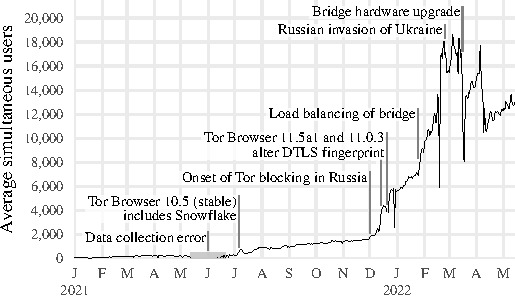
\includegraphics{figures/users-global/users-global}
% TODO: bandwidth chart? ideally with aligned horizontal axis.
\caption{
Estimated average number of simultaneous Snowflake users per day.
The value at the extreme left edge of the graph,
the beginning of 2021, is about~60.
At this point, Snowflake was available in the Tor Browser alpha release series
for desktop platforms and Android,
and it had the Turbo Tunnel session persistence feature.
% Loesing~\cite{tor-tr-2012-10-001} describes how user counts is estimated.
The maximum value in the part of the graph not shown
is 133, on \mbox{2020-12-09}.
% > filtered[which.max(filter(filtered, date < "2021-01-01")$users), ]
% # A tibble: 1 x 4
%   date       transport users  frac
%   <date>     <chr>     <dbl> <dbl>
% 1 2020-12-09 snowflake  133.   100
}
\label{fig:user-counts}
\end{figure}

This brings us to \autoref{fig:user-counts},
which shows the estimated number of Snowflake users since 2021.
Because of Snowflake's affiliation with Tor and Tor Browser,
we estimate users using the normal statistics reported by the bridge
and collected by Tor Metrics.
Be aware: the chart does not show the number of unique daily users,
as one might expect,
but the \emph{average number of simultaneous users} per day.
For example, if the line goes through 1,700 on 2021-12-01,
it means that if the number of Snowflake users were instantaneously sampled
at a random moment in that day, the expected number of users would be 1,700.
The number of unique users per day is necessarily higher,
but how much higher depends on how many hours an average user stays connected.
Counting simultaneous users, rather than unique users,
has been the practice of Tor Metrics since 2012~\cite{tor-tr-2012-10-001};
the reason for it is that the statistics reported by Tor bridges
lend themselves better to the former estimation than the latter.
% TODO: Can we do better with respect to unique users?
% https://bugs.torproject.org/tpo/network-health/metrics/analysis/40012#note_2803514}
The values should not be taken as exact---the
algorithm involves some approximations and guessed parameters---but
the chart is at least relatively comparable to others
produced by Tor Metrics.
% https://bugs.torproject.org/tpo/network-health/metrics/website/40047#note_2796619 "I did some analysis to see what a corrected graph for Snowflake would look like."
% TODO: Speaking of, should we show Snowflake numbers in context with other PTs & relay users?
% https://gitlab.torproject.org/tpo/community/support/-/issues/40050#note_2796770 "This graph shows shows all the Tor users in Russia, whether using relays, bridges, or bridges with pluggable transports."

The growth of Snowflake users began in earnest on
\mbox{2021-07-06}, when it became part of the stable release series
in Tor Browser~10.5.
% https://blog.torproject.org/new-release-tor-browser-105
Being part of the stable series means that it was
available as a built-in option for circumvention for all Tor Browser users,
not only those who had taken the trouble to install a special alpha release.
The rate of adoption increased,
and the number of simultaneous users steadily increased to almost 2,000
over the next five months.

On \mbox{2021-12-01}, some (not all) ISPs in Russia began to block
most forms of access to Tor~\cite{ooni-2021-russia-blocks-tor}.
We will have more to say about this in \autoref{sec:block-ru}.
Snowflake was also affected,
but we released updates to evade the blocking on
\mbox{2021-12-14} (alpha) and
\mbox{2021-12-20} (stable).
The blocking of plain Tor increased demand for circumvention transports,
and Snowflake was strongly affected.
The number of users quadrupled in the next two months.
There were so many new users from Russia, in fact,
that we had to rearchitect the bridge deployment
at the end of January
in order to handle the increased load.
% https://forum.torproject.net/t/tor-relays-how-to-reduce-tor-cpu-load-on-a-single-bridge/1483
% https://bugs.torproject.org/tpo/anti-censorship/pluggable-transports/snowflake/40095#note_2772325
Even with these architectural changes,
the bridge's CPU capacity again became saturated.
Around the beginning of March, Snowflake was almost unusably slow for a few weeks.
% https://old.reddit.com/r/TOR/comments/t49i14/hello_i_have_a_problem_with_snowflake_can_you/
% https://forum.torproject.net/t/tor-project-more-resources-required-for-snowflake-bridge/2353
The invasion of Ukraine by Russia starting on \mbox{2022-03-24}
was accompanied by additional restrictions on Internet access in Russia,
which only increased demand for circumvention.
In response, on \mbox{2022-03-16} we upgraded the bridge to substantial server hardware,
which has been sufficient for the time being.
(See \autoref{sec:future} for an idea to run multiple independent bridge sites,
to permit scaling further.)
As of May 2022, about 65\% of Snowflake users come from Russia.
% https://metrics.torproject.org/collector.html#type-bridge-extra-info
%
% @type bridge-extra-info 1.3
% extra-info flakey3 5481936581E23D2D178105D44DB6915AB06BFB7F
% published 2022-05-20 21:10:47
% transport snowflake
% dirreq-v3-ips ru=12216,us=1640,cn=704,de=400,gb=296,by=272,in=224,??=208,ua=168,fr=160,ir=136,nl=128,ca=88,br=80,it=80,au=72,pl=72,sa=72,es=64,se=64,ch=48,cz=48,mx=48,tr=48,ae=40,jp=40,ro=40,za=40,at=32,eg=32,id=32,co=24,dk=24,dz=24,fi=24,hk=24,hu=24,no=24,ph=24,pk=24,ar=16,bd=16,be=16,cl=16,gr=16,ie=16,il=16,kr=16,kz=16,lt=16,ma=16,mm=16,my=16,ng=16,nz=16,pt=16,sg=16,sk=16,vn=16,al=8,ao=8,az=8,ba=8,bf=8,bg=8,bh=8,bj=8,bo=8,ci=8,cm=8,cr=8,cu=8,cy=8,do=8,ec=8,ee=8,et=8,eu=8,ge=8,gf=8,gh=8,gt=8,hr=8,iq=8,jm=8,jo=8,ke=8,kg=8,km=8,kw=8,lb=8,lk=8,lu=8,lv=8,ly=8,md=8,mk=8,ml=8,mo=8,mu=8,mv=8,mw=8,mz=8,na=8,om=8,pa=8,pe=8,pg=8,pr=8,py=8,qa=8,re=8,rs=8,rw=8,sb=8,sc=8,sd=8,si=8,so=8,sv=8,sy=8,th=8,tm=8,tn=8,tw=8,tz=8,ug=8,uy=8,uz=8,ve=8,ye=8,zm=8
% dirreq-v3-reqs ru=21688,us=2728,cn=1280,de=664,??=648,gb=504,by=464,fr=368,ua=344,in=336,nl=280,ir=248,ca=168,au=152,br=128,it=120,pl=112,es=96,mx=96,ro=96,sa=96,se=88,id=80,ch=72,tr=72,za=72,cz=64,jp=64,ae=56,eg=56,co=48,hk=48,at=40,dk=40,no=40,ar=32,be=32,dz=32,fi=32,ie=32,lv=32,ng=32,nz=32,ph=32,pk=32,pt=32,bd=24,hu=24,il=24,jo=24,kr=24,kz=24,vn=24,az=16,ba=16,cl=16,ec=16,et=16,ge=16,gr=16,hr=16,ke=16,lt=16,ma=16,mm=16,mu=16,my=16,pa=16,sg=16,sk=16,th=16,tm=16,tw=16,uy=16,uz=16,al=8,ao=8,bf=8,bg=8,bh=8,bj=8,bo=8,ci=8,cm=8,cr=8,cu=8,cy=8,do=8,ee=8,eu=8,gf=8,gh=8,gt=8,iq=8,jm=8,kg=8,km=8,kw=8,lb=8,lk=8,lu=8,ly=8,md=8,mk=8,ml=8,mo=8,mv=8,mw=8,mz=8,na=8,om=8,pe=8,pg=8,pr=8,py=8,qa=8,re=8,rs=8,rw=8,sb=8,sc=8,sd=8,si=8,so=8,sv=8,sy=8,tn=8,tz=8,ug=8,ve=8,ye=8,zm=8
% dirreq-v3-resp ok=32240,not-enough-sigs=0,unavailable=0,not-found=0,not-modified=3208,busy=0
% dirreq-v3-direct-dl complete=0,timeout=0,running=0
% dirreq-v3-tunneled-dl complete=27256,timeout=4948,running=32,min=963,d1=112650,d2=280773,q1=417567,d3=637384,d4=13253000,md=22649666,d6=25108500,d7=28307500,q3=31003000,d8=36534666,d9=50908500,max=121278000
% bridge-ips ru=16720,us=2744,cn=1024,de=672,gb=440,by=400,in=400,??=272,fr=264,ua=232,ir=200,nl=200,br=152,ca=152,au=136,it=136,pl=128,sa=112,se=96,tr=96,es=80,jp=80,mx=72,ro=72,ch=64,eg=64,za=64,ae=56,cz=56,at=48,id=48,co=40,dz=40,hk=40,no=40,pk=40,bd=32,be=32,fi=32,kr=32,kz=32,ng=32,pt=32,ar=24,cl=24,dk=24,gr=24,hu=24,ie=24,il=24,ma=24,my=24,ph=24,sk=24,vn=24,bg=16,cu=16,ec=16,gh=16,jo=16,ke=16,kw=16,lk=16,lt=16,lv=16,mm=16,mu=16,nz=16,sg=16,th=16,tw=16,uz=16,ye=16,al=8,ao=8,ap=8,az=8,ba=8,bf=8,bh=8,bj=8,bn=8,bo=8,ci=8,cm=8,cr=8,cy=8,do=8,ee=8,et=8,eu=8,ge=8,gf=8,gn=8,gt=8,hn=8,hr=8,iq=8,is=8,jm=8,kg=8,km=8,lb=8,lu=8,ly=8,md=8,mk=8,ml=8,mo=8,mv=8,mw=8,mz=8,na=8,np=8,om=8,pa=8,pe=8,pg=8,pr=8,ps=8,py=8,qa=8,re=8,rs=8,rw=8,sb=8,sc=8,sd=8,si=8,sn=8,so=8,sr=8,sv=8,sy=8,tm=8,tn=8,tt=8,tz=8,ug=8,uy=8,ve=8,zm=8
% bridge-ip-versions v4=23424,v6=2840
% bridge-ip-transports <OR>=8,snowflake=26264
%
% >>> 21688 / 32240 # dirreq-v3-reqs=ru / dirreq-v3-resp=ok
% 0.6727047146401985
% >>> 16720 / 26264 # bridge-ips=ru / bridge-ip-transports=snowflake
% 0.7137978142076503

% ANON
% The Tor Metrics Timeline~\cite{tor-metrics-timeline}
% has a detailed list of events over the course of Snowflake deployment.

% david
$X$ TB of user data transferred

% cecylia
The deployment of Snowflake proxies began with a bare minimum deployment of three standalone Go proxies all on the same IP address as the Snowflake bridge, as well as a few proxies from deployed Snowflake badges. We began to collect metrics on the number of deployed proxies on \mbox{2019-06-29}. Figure~\ref{fig:total-proxy-counts} shows the total count of unique proxy IP addresses from the beginning of our collection to the writing of this paper. The majority of the growth in Snowflake proxies over the last three years comes from the success of the Snowflake browser add-on. The add-on was released for Firefox on \mbox{2019-06-26} and Chrome on \mbox{2019-07-03}, but the first major spike in proxy counts was thanks to the integration of Snowflake with the existing flash proxy add-on, Cupcake. The number of Cupcake proxies dropped off completely later that year, but Snowflake add-on usage had already risen to compensate. Currently, the vast majority of Snowflake proxies are from the browser add-on, as shown in Figure~\ref{fig:proxy-type-counts}.

While early growth in the number of unique Snowflake proxy IPs was due to the development of easier deployment methods and UX features for proxy volunteers, the later growth in proxy counts were due to outreach and follow the increase in demand for Snowflake proxy capacity from the increase in client usage. 

Counts of web badge vs. browser add-on vs. standalone daemon
Timeline of proxy + webext deployment
% |2019-06-26|||snowflake|Deployed version 0.0.1 of the Snowflake WebExtension for Firefox.|[comment](https://bugs.torproject.org/tpo/anti-censorship/pluggable-transports/snowflake/30931#note_2593598)||
% |2019-07-03|||snowflake|Deployed version 0.0.1 of the Snowflake WebExtension for Chrome.|[comment](https://bugs.torproject.org/tpo/anti-censorship/pluggable-transports/snowflake/30999#note_2593718)||
Cupcake
Relative ineffectiveness of web badge (i.e. the flash proxy model)
people love the add-on and the daily count of connections

Orbot? as both client and proxy?

\subsection{Development challenges}

% arlo, cecylia

Difficulty of using WebRTC outside a browser

Reproducible builds
- difficulty of cross-compiling go-webrtc extracted from Chromium

scaling
% david
- load balancing
- multi-bridge

% Safe Browsing / zip bomb problem (2019)
% https://gitlab.torproject.org/tpo/anti-censorship/pluggable-transports/snowflake/-/issues/31250


\subsection{Blocking in Turkmenistan}
\label{sec:block-tm}

\begin{figure}
\framebox[\linewidth]{\vbox to 2in{\vfil\centering TODO\vfil}}
\caption{
Users in Turkmenistan and Russia,
around blocking events.
}
\label{fig:user-counts-tm-ru}
\end{figure}

% |2021-10-24||tm|snowflake|Snowflake users in Turkmenistan drop to zero, possibly as a result of blocking of the broker's domain-fronting channel.|[issue](https://bugs.torproject.org/tpo/anti-censorship/censorship-analysis/40024) [comment](https://bugs.torproject.org/tpo/community/support/40030#note_2759213) [discussion](http://meetbot.debian.net/tor-meeting/2021/tor-meeting.2021-11-04-15.59.log.html#l-55)|X|

\url{https://bugs.torproject.org/tpo/anti-censorship/censorship-analysis/40024}

\autoref{fig:user-counts-tm-ru}

Block of domain front
Unclear if AMP cache rendezvous was a sufficient workaround
Hard to get testers/volunteers

\subsection{Blocking in Russia}
\label{sec:block-ru}

% https://gitlab.torproject.org/tpo/community/support/-/issues/40050#note_2796770

% mention the creeping block of VPNs? https://github.com/net4people/bbs/issues/76

% david

\autoref{fig:user-counts-tm-ru}

\url{https://bugs.torproject.org/tpo/community/support/40050}
\url{https://ntc.party/t/ooni-reports-of-tor-blocking-in-certain-isps-since-2021-12-01/1477}
% \url{https://blog.torproject.org/tor-censorship-in-russia/}

Snowflake blocked in Russia, along with all other Tor protocols,
in December 2021 \cite{ooni-2021-russia-blocks-tor}
In comparison to TM, easy to get testers
Managed to unblock it within 2 weeks

supported\_groups in Specific DTLS Server Hello Extension
Release to change fingerprint evaded blocking, has worked in Russia since
Had been anticipated by MacMillan et al.\cite[\S 3]{arxiv.2008.03254}
Though not necessarily the wrong call not to have prioritized a fix earlier
Importance during the invasion of Ukraine
- increased usage caused scaling difficulties
  \url{https://forum.torproject.net/t/tor-project-more-resources-required-for-snowflake-bridge/2353}

Second round of DTLS fingerprinting, this time targeting DTLS Client Hello?
\url{https://bugs.torproject.org/tpo/anti-censorship/censorship-analysis/40030#note_2803188}
\url{https://bugs.torproject.org/tpo/anti-censorship/pluggable-transports/snowflake/40140}
\url{https://ntc.party/t/a-new-snowflake-blocking-rule-offset-of-supported-groups-in-dtls-client-hello/2420}

\subsection{SQL injection attempts at broker}

% cecylia

\url{https://bugs.torproject.org/tpo/anti-censorship/pluggable-transports/snowflake/40089}
Actually tailored to the broker protocol, not a generic attack tool.

\subsection{Rate of proxy IP address churn}

% shelikhoo

Need a new experiment for this
\url{https://bugs.torproject.org/tpo/anti-censorship/pluggable-transports/snowflake/34075}

\subsection{Performance}
\label{sec:performance}

% cecylia

\section{Future work}
\label{sec:future}

% shelikhoo

Distributed bridge architecture
\url{https://bugs.torproject.org/tpo/anti-censorship/pluggable-transports/snowflake/40129}

% ANON
% \section*{Availability}
%
% \url{https://snowflake.torproject.org/}

% ANON
% \section*{Acknowledgements}
%
% Griffin Boyce
% Chris Ball
% Tor Project
% Sukhbir Singh
% Ivan Markin (AMP cache)
% Pion (who at Pion?)
% ValdikSS (fingerprinting research during Russia blocking)
% Vern Paxson, CDT, OTF, anyone else Serene was involved with?
% Greenhost (eclips.is)
% Arthur Edelstein
% Linus Nordberg
% Mullvad (donated bridge hardware)
% volunteers running snowflake proxies
% anonymous donors

\bibliographystyle{plainurl}
\bibliography{snowflake}

\end{document}
